\documentclass[12pt,a4paper]{report}

\usepackage[margin=1in]{geometry}
\usepackage{graphicx}
\usepackage{array}
\usepackage{booktabs}
\usepackage{float}
\usepackage{setspace}
\usepackage{titlesec}
\usepackage{tocloft}
\usepackage{enumitem}
\usepackage{hyperref}
\usepackage{xcolor}
\usepackage{url}
\usepackage{eso-pic}
\usepackage{tikz}
\usepackage{fancyhdr}
\usepackage{lastpage}
\usepackage{etoolbox}

\hypersetup{
    colorlinks=true,
    linkcolor=black,
    urlcolor=blue,
    pdftitle={Internship Report},
    pdfauthor={Keerthana C}
}

% -- Spacing ----------------------------------------------------------------
\setstretch{1.5}
\setlength{\parindent}{1.5em}
\setlength{\parskip}{0.4em}

% -- Chapter heading format -------------------------------------------------
\titleformat{\chapter}[display]
  {\filcenter\bfseries\Large}
  {\chaptername~\thechapter}{10pt}{\LARGE\markboth{\MakeUppercase{##1}}{\MakeUppercase{##1}}}

% Ensure chapter marks are set for headers
\renewcommand{\chaptermark}[1]{\markboth{##1}{##1}}

% -- Rename TOC / LOF headings to match template ----------------------------
\renewcommand{\contentsname}{TABLE OF CONTENTS}
\renewcommand{\listfigurename}{LIST OF FIGURES}

% -- TOC heading format (consistent with other front-matter headings) -------
\renewcommand{\cfttoctitlefont}{\hfill\LARGE\bfseries}
\renewcommand{\cftaftertoctitle}{\hfill}
\renewcommand{\cftloftitlefont}{\hfill\LARGE\bfseries}
\renewcommand{\cftafterloftitle}{\hfill}
\setlength{\cftbeforetoctitleskip}{-1.5em}
\setlength{\cftaftertoctitleskip}{1.5em}
\setlength{\cftbeforeloftitleskip}{-1.5em}
\setlength{\cftafterloftitleskip}{1.5em}
\renewcommand{\cftsecleader}{\cftdotfill{\cftdotsep}}
\renewcommand{\cftchapleader}{\cftdotfill{\cftdotsep}}

% -- Toggle: border ON/OFF --------------------------------------------------
% We define a boolean that controls whether borders are drawn.
% Front-matter pages: border ON.  Chapter pages: border OFF.
\newif\ifshowborder
\showbordertrue  % start with borders ON

\AddToShipoutPictureBG{%
  \ifshowborder
  \begin{tikzpicture}[remember picture, overlay]
    \draw[line width=0.56pt]
      ([xshift=18pt, yshift=-18pt]current page.north west)
      rectangle
      ([xshift=-18pt, yshift=18pt]current page.south east);
    \draw[line width=0.28pt]
      ([xshift=20pt, yshift=-20pt]current page.north west)
      rectangle
      ([xshift=-20pt, yshift=20pt]current page.south east);
  \end{tikzpicture}%
  \fi
}

% -- Page styles ------------------------------------------------------------

% Style for front-matter: no header/footer, just centered page number
\fancypagestyle{frontmatter}{
  \fancyhf{}
  \renewcommand{\headrulewidth}{0pt}
  \renewcommand{\footrulewidth}{0pt}
  \fancyfoot[C]{\thepage}
}

% Style for main content: header + footer, no border
\fancypagestyle{mainchapter}{
  \fancyhf{}
  \renewcommand{\headrulewidth}{0.4pt}
  \renewcommand{\footrulewidth}{0.4pt}
  \fancyhead[L]{\small Developer}
  \fancyhead[R]{\small\nouppercase{\leftmark}}
  \fancyfoot[L]{\small Dept. of ECE, Vemana IT}
  \fancyfoot[C]{\small 2025-2026}
  \fancyfoot[R]{\small Page \thepage\ of \pageref{LastPage}}
  \renewcommand{\chaptermark}[1]{\markboth{##1}{}}
}

% Plain style for front-matter (used by \chapter*, \listoffigures, etc.)
% Initially just centered page number. Redefined before main content.
\fancypagestyle{plain}{
  \fancyhf{}
  \renewcommand{\headrulewidth}{0pt}
  \renewcommand{\footrulewidth}{0pt}
  \fancyfoot[C]{\thepage}
}

\begin{document}

% ==========================================================================
% TITLE PAGE  (single-spaced, zero parskip so it fits on one page)
% ==========================================================================
\begin{titlepage}
\thispagestyle{empty}
\begin{singlespacing}
\setlength{\parskip}{0pt}
\setlength{\parindent}{0pt}
\centering
\vspace*{-0.5cm}

{\Large \textbf{VISVESVARAYA TECHNOLOGICAL UNIVERSITY}\par}
\vspace{2pt}
{\large \textbf{Jnana Sangama, Belagavi -- 590018}\par}
\vspace{8pt}

\includegraphics[height=5cm]{images/vtu_logo.png}\par
\vspace{8pt}
{\itshape An Internship Report\par}
\vspace{2pt}
{\itshape On\par}
\vspace{4pt}
{\LARGE \textbf{\textquotedblleft Developer\textquotedblright}\par}
\vspace{4pt}
{\textcolor{red}{Feb 2 to May 2}\par}
\vspace{8pt}
{\itshape Submitted in partial fulfillment of the requirements for the award of the degree of\par}
\vspace{4pt}
{\large \textbf{Bachelor of Engineering}\par}
\vspace{2pt}
{\large \textbf{in}\par}
\vspace{2pt}
{\large \textbf{\textcolor{blue}{Electronics and communication Engineering}}\par}
\vspace{8pt}
Submitted by\par
\vspace{4pt}
{\large \textbf{KEERTHANA C \hspace{2cm} 1VI22EC072}\par}
\vspace{10pt}

\includegraphics[height=4cm]{images/vit_logo.png}\par
\vspace{10pt}
{\large \textbf{DEPARTMENT OF ELECTRONICS AND COMMUNICATION ENGINEERING}\par}
{\Large \textbf{VEMANA INSTITUTE OF TECHNOLOGY}\par}
{\large BENGALURU -- 560034\par}
\vspace{6pt}
{\Large \textbf{2025-2026}\par}

\end{singlespacing}
\end{titlepage}

% ==========================================================================
% FRONT MATTER — borders ON, roman numbering, no headers/footers
% ==========================================================================
\pagenumbering{roman}
\pagestyle{frontmatter}

% ==========================================================================
% CERTIFICATE PAGE
% ==========================================================================
\thispagestyle{empty}
\begin{singlespacing}
\setlength{\parskip}{0pt}
\setlength{\parindent}{0pt}
\begin{center}
{\large \textbf{Karnataka ReddyJana Sangha}\par}
\vspace{2pt}
{\Large \textbf{VEMANA INSTITUTE OF TECHNOLOGY}\par}
\vspace{2pt}
(Affiliated to Visvesvaraya Technological University, Belagavi)\par
Koramangala, Bengaluru--560034\par
\vspace{8pt}

\includegraphics[height=3.5cm]{images/dept_seal.png}\par
\vspace{10pt}
{\large \textbf{DEPARTMENT OF}\par}
{\large \textbf{ELECTRONICS AND COMMUNICATION ENGINEERING}\par}
\vspace{10pt}
\addcontentsline{toc}{chapter}{Certificate}
{\LARGE \textbf{CERTIFICATE}\par}
\end{center}
\end{singlespacing}

\vspace{6pt}
\setlength{\parindent}{1.5em}
This is to certify that the internship entitled \textbf{\textquotedblleft Developer\textquotedblright} is a bonafide work carried out by \textbf{KEERTHANA C (1VI22EC072)} in partial fulfilment of the requirements for the award of Bachelor of Engineering degree in \textbf{Electronics and communication Engineering}, Visvesvaraya Technological University, Belagavi, during the academic year 2025-2026.

It is certified that all corrections and suggestions indicated for internal assessment have been duly incorporated in the report. The internship report has been approved as it satisfies the academic requirements prescribed for the said degree.

% -- Watermark: VIT logo behind signatures ---------------------------------
\AddToShipoutPictureFG*{%
  \begin{tikzpicture}[remember picture, overlay]
    \node[opacity=0.10] at ([yshift=-4cm]current page.center) {%
      
\includegraphics[height=8cm]{images/vit_logo.png}%
    };
  \end{tikzpicture}%
}

\vspace{0.6cm}
\begin{center}
\begin{tabular}{>{\raggedright\arraybackslash}p{0.23\textwidth} >{\raggedright\arraybackslash}p{0.24\textwidth} >{\raggedright\arraybackslash}p{0.20\textwidth} >{\raggedright\arraybackslash}p{0.23\textwidth}}
\textbf{Internal Supervisor} & \textbf{External Supervisor} & \textbf{HOD} & \textbf{Principal} \\
(Prof. Suma B V) & (N. Vijay Anand) & (Dr. Suneeta) & (Dr. Vijayasimha Reddy B G) \\
\end{tabular}
\end{center}

\vspace{0.5cm}
\textbf{Name of the Examiners} \hfill \textbf{Signature with Date}\par
\vspace{0.2cm}
1.\enspace\rule{5cm}{0.4pt} \hfill \rule{3.5cm}{0.4pt}\par
\vspace{0.4cm}
2.\enspace\rule{5cm}{0.4pt} \hfill \rule{3.5cm}{0.4pt}\par


\newpage
\begin{center}
\vspace*{\fill}
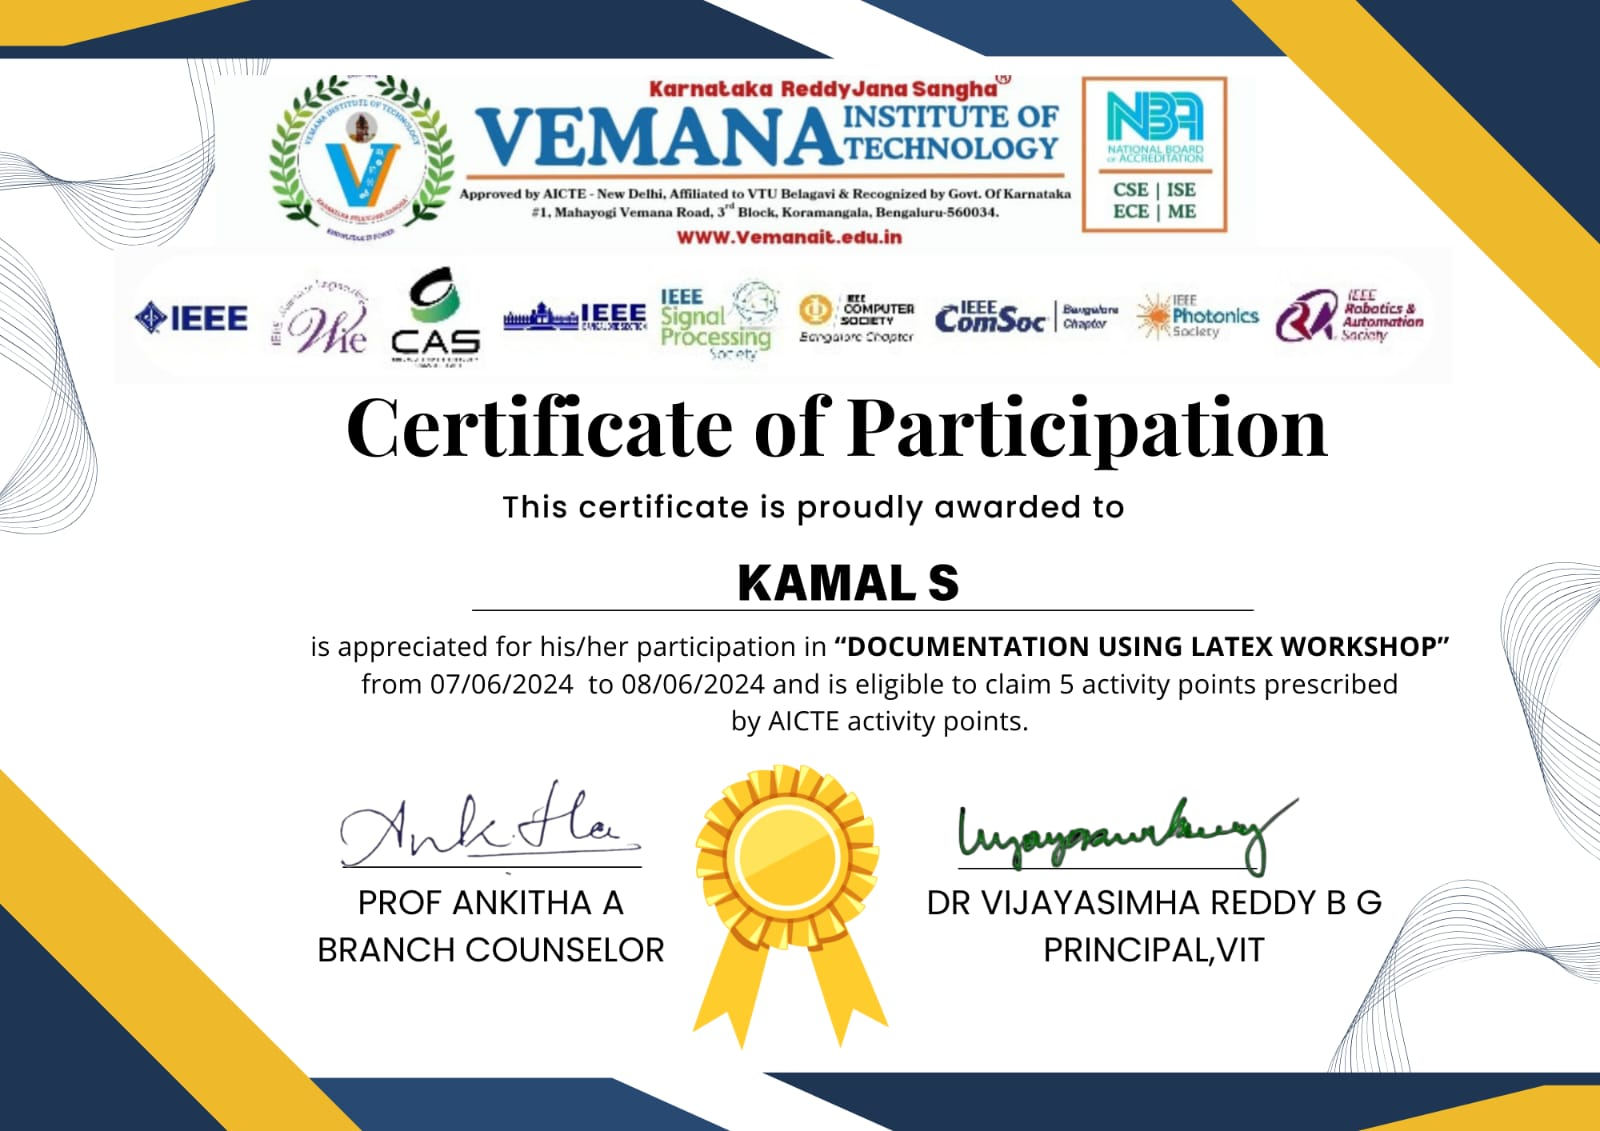
\includegraphics[angle=90,origin=c,width=0.92\textheight,height=0.92\textwidth,keepaspectratio]{images/cert_image_08b1baed.jpeg}
\vspace*{\fill}
\end{center}


% ==========================================================================
% ACKNOWLEDGEMENT
% ==========================================================================
\newpage
\setcounter{page}{2}  % Ack = page ii (certificate was empty)
\begin{center}
{\LARGE \textbf{ACKNOWLEDGEMENT}\par}
\end{center}
\addcontentsline{toc}{chapter}{Acknowledgement}

\vspace{0.5cm}
\setlength{\parskip}{1em}
\begin{onehalfspacing}

I would like to express my sincere gratitude to Visvesvaraya Technological University (VTU) for providing me with the opportunity to undertake this internship as a part of my academic curriculum. I extend my heartfelt thanks to the Principal of Vemana Institute of Technology, Dr. Vijayasimha Reddy B G, for his constant support and encouragement throughout my academic journey.


I am deeply thankful to the Head of the Department, Dr. Suneeta, for her valuable guidance and motivation. I would also like to express my sincere appreciation to my internal supervisor, Prof. Suma B V, for her continuous support, constructive feedback, and encouragement during the internship period.


I would like to extend my special thanks to my external supervisor, Mr. N. Vijay Anand from TriSpace Technologies, for providing me with the opportunity to work on real-time DSP systems and for guiding me throughout the internship. His technical insights and mentorship played a crucial role in enhancing my understanding of embedded systems and DSP programming.


I would also like to thank all the staff members at TriSpace Technologies for their support, knowledge sharing, and collaborative environment, which made my learning experience highly enriching.


Finally, I would like to express my gratitude to my family and friends for their constant encouragement and support throughout this internship.

\end{onehalfspacing}
\setlength{\parskip}{0.4em}

\vspace{1cm}
\begin{flushright}
\textbf{Keerthana C}\par
1VI22EC072\par
\end{flushright}

% ==========================================================================
% ABSTRACT
% ==========================================================================
\newpage
\begin{center}
{\LARGE \textbf{ABSTRACT}\par}
\end{center}
\addcontentsline{toc}{chapter}{Abstract}

\vspace{0.5cm}
\setlength{\parindent}{1.5em}

During my internship at TriSpace Technologies, I worked in the role of a Developer, focusing on Digital Signal Processing (DSP) and embedded system programming using Qualcomm Snapdragon System-on-Chip (SoC) platforms. The internship was designed to provide hands-on exposure to real-time signal processing, low-level programming, and performance optimization techniques used in industry-level systems.


Throughout the internship, I gained in-depth knowledge of processor-level architecture, particularly the Qualcomm Hexagon DSP. I implemented various algorithms using both C programming and assembly language, which enabled me to understand the execution flow from high-level logic to low-level instruction mapping. My work included developing and optimizing arithmetic operations, logical operations, vector instructions, and core DSP functions such as Multiply-Accumulate (MAC) and maximum search.


A significant portion of my internship involved working with DSP-specific tools such as syn\_fit and build\_code for analyzing, compiling, and optimizing algorithms. I also explored advanced signal processing modules including Automatic Gain Control (AGC), Codebook Search (CBSearch), and residue computation. These tasks helped me understand how real-time systems maintain performance while minimizing power consumption.


The internship followed a structured approach involving learning, implementation, debugging, and optimization. I developed strong analytical and problem-solving skills while working on complex DSP operations and debugging low-level code.


Overall, this internship significantly enhanced my technical knowledge in embedded systems and DSP programming, bridging the gap between academic theory and industrial practice.


Strong line: 👉 “This internship transformed my understanding of DSP from theoretical concepts into high-performance, real-time embedded implementations.”


% ==========================================================================
% TABLE OF CONTENTS — Standard LaTeX TOC with dotted leaders
% ==========================================================================
\newpage
\tableofcontents

% ==========================================================================
% LIST OF FIGURES — Custom table format matching template
% ==========================================================================
\newpage
% We need the custom header for LOF
\addtocontents{lof}{\textbf{Figure No} \hfill \textbf{Title} \hfill \textbf{Page No}\par\smallskip\hrule\par\bigskip}
\listoffigures

% ==========================================================================
% MAIN CONTENT — borders OFF, headers/footers ON, arabic numbering
% ==========================================================================
\newpage
\showborderfalse       % TURN OFF borders for all remaining pages
\pagenumbering{arabic}

% Redefine plain style for chapter first pages — SAME as mainchapter
% Template shows header + footer on ALL chapter pages including the first page
\fancypagestyle{plain}{
  \fancyhf{}
  \renewcommand{\headrulewidth}{0.4pt}
  \renewcommand{\footrulewidth}{0.4pt}
  \fancyhead[L]{\small Developer}
  \fancyhead[R]{\small\nouppercase{\leftmark}}
  \fancyfoot[L]{\small Dept. of ECE, Vemana IT}
  \fancyfoot[C]{\small 2025-2026}
  \fancyfoot[R]{\small Page \thepage\ of \pageref{LastPage}}
  \renewcommand{\chaptermark}[1]{\markboth{##1}{}}
}
\pagestyle{mainchapter}

% ==========================================================================
% CHAPTER 1: INTRODUCTION
% ==========================================================================
\chapter{INTRODUCTION}
\label{ch:intro}


The internship at TriSpace Technologies, where I worked as a Developer, provided me with an opportunity to gain practical experience in Digital Signal Processing (DSP) and embedded system development. In today’s rapidly evolving technological landscape, internships play a vital role in bridging the gap between theoretical learning and real-world application, especially in core engineering domains such as Electronics and Communication Engineering.


This chapter introduces the scope, objectives, and relevance of the internship. It highlights the importance of DSP programming in modern systems, including mobile devices and communication systems, where performance and efficiency are critical. The chapter also discusses how the field has evolved over time and the current trends shaping the industry.


Through this internship, I was able to understand how low-level programming and optimization techniques contribute to efficient system design. This chapter provides a foundation for the detailed discussions presented in the subsequent chapters, including the organizational profile, work methodology, results, and conclusions.


\section{Internship Scope and Objectives}

The primary objective of my internship at TriSpace Technologies was to gain practical knowledge in DSP programming and embedded system development while working on real-world applications using Qualcomm Snapdragon platforms.


The scope of the internship included both technical and professional development, focusing on the following objectives:


Understanding DSP Fundamentals I aimed to build a strong foundation in Digital Signal Processing concepts, including signal representation, filtering, and algorithm design. Learning C Programming for Embedded Systems I worked on developing efficient C programs to understand logical flow and prepare for low-level implementation. Assembly-Level Programming A key objective was to convert high-level C code into assembly instructions for the Hexagon DSP, improving understanding of processor-level execution. Implementation of DSP Algorithms I implemented core DSP operations such as MAC, vector operations, and maximum search algorithms used in real-time systems. Performance Optimization I focused on optimizing algorithms using DSP-specific instructions to improve execution speed and reduce power consumption. Tool Utilization Learning tools such as syn\_fit and build\_code was essential for analyzing and optimizing DSP algorithms. Debugging and Testing I developed skills in debugging low-level code and analyzing outputs for correctness and efficiency. Professional Development The internship aimed to enhance problem-solving skills, analytical thinking, and time management.


Overall, the internship scope was designed to provide a comprehensive understanding of DSP systems from both theoretical and practical perspectives.


\section{Relevance of Developer to Electronics and communication Engineering}

The role of a Developer in DSP and embedded systems is highly relevant to Electronics and Communication Engineering (ECE), as it directly aligns with core subjects and practical applications studied during the course.


Firstly, the internship reinforced concepts from Digital Signal Processing, where I applied theoretical knowledge of signals, filters, and transforms into practical implementations. Understanding operations such as MAC and vector processing provided deeper insight into real-time signal computation.


Secondly, the internship was closely related to Microprocessors and Microcontrollers, as it involved programming at the processor level. Writing assembly code for the Hexagon DSP enhanced my understanding of instruction sets, memory management, and execution flow.


Thirdly, the work aligned with Embedded Systems Design, where hardware and software integration plays a critical role. Implementing algorithms on Qualcomm Snapdragon platforms helped me understand system-level design and constraints.


Additionally, concepts from Communication Systems were indirectly applied, particularly in functions such as AGC and CBSearch, which are used in signal transmission and processing.


Finally, the internship strengthened my knowledge in VLSI and Computer Architecture, as it involved understanding processor pipelines, parallel execution, and optimization techniques.


Thus, the internship provided a strong connection between academic coursework and real-world engineering applications.


\section{Evolution of Practices in the Field}

The field of Digital Signal Processing (DSP) and embedded systems has undergone significant transformation over the past few decades, evolving from basic computation models to highly optimized and parallel processing architectures.


In the early stages, signal processing was primarily implemented using analog systems. These systems were limited in flexibility and accuracy, as modifying the behavior required hardware changes. With the introduction of digital systems, signal processing began to shift towards software-based implementations using general-purpose processors.


The next major phase involved the development of dedicated DSP processors. These processors were specifically designed to handle signal processing tasks efficiently, introducing features such as Multiply-Accumulate (MAC) units and specialized instruction sets. This significantly improved performance in applications such as audio and communication systems.


With advancements in semiconductor technology, System-on-Chip (SoC) architectures emerged, integrating multiple processing units into a single chip. Platforms such as Qualcomm Snapdragon introduced specialized DSP cores like the Hexagon DSP, enabling parallel processing and vector operations.


In the current phase, DSP systems are highly optimized for real-time processing, low power consumption, and high performance. The integration of AI and machine learning with DSP has further expanded its applications in areas such as image processing, speech recognition, and autonomous systems.


Thus, the evolution of DSP reflects a shift from hardware-dependent systems to highly flexible, software-driven, and performance-optimized architectures.


The evolution of practices in the field of Developer has been marked by significant advancements in technology and methodology. Early approaches relied heavily on manual processes and standalone systems. With the advent of the internet and cloud computing, the field shifted towards distributed systems and web-based solutions. Modern practices now emphasize automation, continuous integration, and agile development methodologies. The integration of artificial intelligence and machine learning has further transformed the landscape, enabling predictive analytics, intelligent automation, and data-driven decision making. These advancements have made it essential for professionals to continuously update their skills and adapt to emerging technologies.


Furthermore, the transition from monolithic architectures to microservices has radically changed how software and hardware systems are designed and maintained. This architectural shift allows teams to work independently, accelerating the delivery of complex features. It also requires a robust understanding of containerization, orchestration tools, and distributed system debugging. In the current industry scenario, keeping abreast with these evolutionary steps is crucial for delivering high-performance, resilient, and scalable solutions that meet modern business demands.


\section{Current Trends and Technologies}

The field of DSP and embedded systems is continuously evolving, with several modern trends shaping its development and applications.


One of the key trends is parallel processing and vectorization, where multiple data elements are processed simultaneously. This is widely used in DSP architectures like the Hexagon DSP to improve performance and efficiency.


Another important trend is low-power optimization, which is critical in mobile and embedded devices. Techniques such as efficient instruction usage, clock gating, and algorithm-level optimization are used to reduce power consumption.


The integration of Artificial Intelligence (AI) with DSP is also gaining importance. DSP processors are now being used to accelerate AI workloads such as speech recognition and image processing in real-time systems.


Hardware-software co-design is another emerging trend, where both hardware and software are optimized together to achieve better system performance. This approach is widely used in embedded system development.


Additionally, the use of advanced development tools such as syn\_fit and build\_code enables efficient analysis, optimization, and debugging of DSP algorithms.


Finally, real-time processing systems are becoming increasingly important, especially in applications such as communication systems, IoT devices, and multimedia processing.


These trends highlight the importance of continuous learning and adaptation in the field of DSP and embedded systems.


🔷 CHAPTER 2: ORGANISATION PROFILE


Several key trends are shaping the current landscape of Developer. Cloud-native development and microservices architecture have become standard practices for building scalable applications. DevOps practices and CI/CD pipelines have streamlined the software development lifecycle. The adoption of containerization technologies such as Docker and Kubernetes has revolutionized deployment strategies. Edge computing is gaining traction for applications requiring low-latency processing.


Furthermore, the increasing emphasis on cybersecurity has led to the adoption of security-first development practices across organizations of all sizes. The rise of generative AI and automated coding assistants is another massive trend, significantly reducing the boilerplate code developers write and shifting the focus to high-level architecture and problem-solving. Teams are also exploring sustainable and green computing, optimizing algorithms to reduce energy consumption, which is becoming a priority for global enterprises.




% ==========================================================================
% CHAPTER 2: ORGANISATION PROFILE
% ==========================================================================
\chapter{ORGANISATION PROFILE}
\label{ch:org}


This chapter provides an overview of TriSpace Technologies, the organization where I completed my internship as a Developer. Understanding the organization is essential to gain context about the work environment, technological focus, and industry relevance of the internship.


The chapter includes details about the company’s background, vision and mission, programs and services offered, organizational impact, and core values. It also highlights how the company contributes to the field of embedded systems and DSP technologies.


By understanding the structure and objectives of TriSpace Technologies, I was able to better align my learning and work with industry expectations and standards.


\section{Introduction}

TriSpace Technologies is a deep-tech organization specializing in advanced domains such as Digital Signal Processing (DSP), embedded systems, and Qualcomm platform development. With over a decade of experience in the field, the company has established itself as a strong contributor to industry-oriented training and technology development.


The organization focuses on bridging the gap between academic learning and industry requirements by providing practical, hands-on experience in real-world systems. It primarily serves students, professionals, and organizations seeking expertise in embedded systems and signal processing technologies.


TriSpace Technologies is particularly known for its work with Qualcomm Snapdragon System-on-Chip (SoC) platforms and Hexagon DSP architectures. These platforms are widely used in modern mobile devices and require specialized programming techniques for efficient performance and power optimization.


The company offers a combination of training programs and development services, enabling learners to gain both conceptual knowledge and practical implementation skills. Its training modules are designed to simulate real-world engineering challenges, helping students develop problem-solving abilities and technical expertise.


Over the years, TriSpace Technologies has built a reputation for delivering high-quality technical training and solutions. Its focus on low-level programming, hardware-software integration, and real-time processing makes it a valuable contributor to the embedded systems ecosystem.



\begin{figure}[H]
\centering

\includegraphics[width=0.55\textwidth,height=5cm,keepaspectratio]{images/company_logo_4d5dc9fd.png}
\caption{Internship Provider - TriSpace Logo}
\end{figure}


\section{Vision and Mission of the Organization}

Vision


The vision of TriSpace Technologies is to become a leading organization in the field of embedded systems and DSP technologies by delivering innovative and efficient solutions that meet modern technological demands. The company aims to contribute to advancements in processor-level programming, signal processing, and system optimization.


It also focuses on building a strong learning ecosystem where students and professionals can acquire industry-relevant skills and effectively solve real-world engineering problems.


Mission


The mission of TriSpace Technologies is to provide high-quality training and development opportunities in advanced technological domains such as DSP programming, embedded systems, and hardware-software integration.


The organization aims to:


Deliver practical and industry-oriented training programs Enhance technical skills in low-level programming and optimization Promote innovation in signal processing techniques Prepare students for careers in core engineering domains


These vision and mission statements directly influence the work culture, emphasizing hands-on learning, innovation, and technical excellence.


The organization's vision extends to becoming a leading provider of technology solutions that drive innovation and create lasting value for clients and stakeholders. Their mission emphasizes the importance of continuous learning, practical skill development, and maintaining the highest standards of quality in all deliverables. This alignment between vision and daily practice creates a productive and growth-oriented work environment.


Looking forward, the organization aims to expand its technological footprint by embracing open-source initiatives and community-driven projects. They emphasize fostering a workplace culture where ethical engineering and societal impact are at the forefront of every business decision. This forward-thinking vision ensures they remain competitive while contributing positively to the broader technology ecosystem.


\section{Programs and Services Offered}

TriSpace Technologies offers a wide range of programs and services aimed at developing technical expertise in embedded systems and DSP domains.


DSP Programming Training This program focuses on signal processing algorithms, vector operations, and optimization techniques using Qualcomm Hexagon DSP. Embedded Systems Development Provides knowledge on microcontrollers, processors, and real-time system design, including hardware-software integration. Qualcomm Platform Training Offers hands-on experience with Snapdragon SoC platforms, including working with DSP cores and optimization tools. Low-Level Programming Covers C programming and assembly programming with a focus on processor-level understanding and performance optimization. Internship Programs Structured internships designed to provide real-time exposure to industry-level projects and workflows. Algorithm Optimization Services Focuses on improving execution efficiency and reducing power consumption in DSP-based applications.


These programs ensure that learners are equipped with both theoretical knowledge and practical skills required in the industry.


The organization offers a diverse range of programs and services that cater to various aspects of technology and engineering. These include structured internship programs for engineering students, professional training workshops, consulting services for technology implementation, and research and development initiatives. The programs are designed to bridge the gap between academic knowledge and industry requirements, ensuring that participants gain practical, applicable skills.


In addition to technical skill development, the organization conducts seminars on leadership, project management, and agile methodologies. This holistic approach ensures that individuals are well-equipped to handle the multifaceted challenges of the modern corporate world. Their services are continually updated to reflect the latest technological advancements, ensuring clients and students receive the most current and relevant guidance.


\section{Organizational Impact and Reach}

TriSpace Technologies has made a significant impact in the field of embedded systems and DSP training by contributing to both education and industry.


Some of the key impact areas include:


Training a large number of engineering students in DSP and embedded systems Bridging the gap between academic curriculum and industry requirements Providing hands-on experience with real-world tools and platforms Enhancing employability of students in core engineering domains Contributing to research and innovation in signal processing techniques Supporting professionals in upgrading their technical skills


The organization plays a crucial role in developing skilled engineers who are capable of working on advanced technological systems.


The organization has made a significant impact in the technology sector through its commitment to quality, innovation, and skill development. Key impact areas include training and mentoring hundreds of engineering students, developing solutions that improve operational efficiency for client organizations, contributing to open-source projects and knowledge sharing, and establishing partnerships with academic institutions. These efforts have positioned the organization as a trusted partner in the technology ecosystem.


Their commitment to excellence has resulted in several industry accolades and a high retention rate among their client base. By continuously delivering scalable and reliable technological solutions, they have empowered businesses to achieve their digital transformation goals faster and more efficiently. Furthermore, their internship programs have successfully transitioned many students into highly skilled professionals, significantly reducing the industry's skill gap.


\section{Core Values}

TriSpace Technologies operates based on strong core values that guide its approach to learning and innovation.


Innovation The company encourages the development of new ideas and advanced solutions in DSP and embedded systems. Technical Excellence High standards are maintained in programming, design, and system optimization to ensure quality output. Practical Learning Emphasis is placed on hands-on experience and real-world applications rather than purely theoretical knowledge. Industry Relevance Training programs are aligned with current industry requirements and emerging technologies. Continuous Improvement The organization promotes constant learning and skill development to keep up with technological advancements. Collaboration Teamwork and knowledge sharing are encouraged to enhance learning and productivity. Integrity Ethical practices and professionalism are maintained in all activities. Commitment to Quality The company ensures high-quality training and project execution.


These values are reflected in the daily work culture, creating a strong learning environment for interns and professionals.


🔷 CHAPTER 3: WORK DONE / METHODOLOGY


These core values are not merely stated principles but are actively embedded in the organization's daily operations, decision-making processes, and employee interactions. The commitment to these values creates a work culture that fosters creativity, encourages continuous improvement, and supports both individual and collective growth.


Transparency, integrity, and collaboration form the foundation of their corporate philosophy. Employees are encouraged to take ownership of their work and are provided with the autonomy to experiment with novel solutions. This environment not only accelerates innovation but also ensures that ethical considerations and high quality standards are maintained across all projects and deliverables.



\begin{figure}[H]
\centering
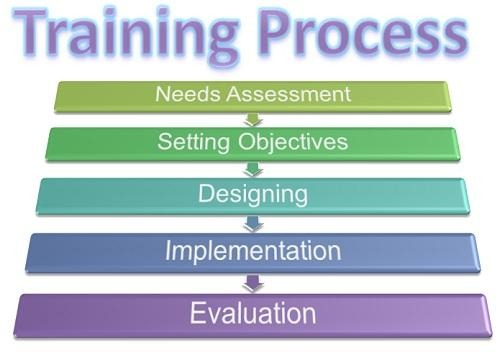
\includegraphics[width=0.45\textwidth,height=5cm,keepaspectratio]{images/ch_img_e16fa761.jpeg}
\caption{Training process}
\end{figure}


% ==========================================================================
% CHAPTER 3: WORK DONE / METHODOLOGY
% ==========================================================================
\chapter{WORK DONE / METHODOLOGY}
\label{ch:work}


This chapter presents a detailed description of the work carried out during my internship at TriSpace Technologies in the role of a Developer. The internship followed a structured progression, starting from fundamental programming concepts and gradually advancing towards complex DSP algorithm implementation and optimization.


The overall workflow of the internship can be divided into multiple phases, including learning basic C programming, transitioning to assembly-level programming, implementing DSP-specific operations, and finally optimizing algorithms using specialized tools. Each phase was designed to build upon the previous one, ensuring a clear understanding of both theoretical and practical aspects.


The chapter also covers the tools and technologies used, the methodology followed during development, and a detailed case study of a key project. Additionally, it highlights the challenges faced during the internship and the solutions implemented to overcome them.


\section{Overview of Internship Work}

During my internship at TriSpace Technologies, I was actively involved in multiple technical tasks related to DSP programming and embedded system development. My daily work was structured into different phases, each focusing on specific learning and implementation goals.


Phase 1: Foundation Building (C Programming) Initially, I worked on basic C programming concepts to build a strong foundation. This included writing programs for arithmetic operations, logical operations, and understanding control structures. These exercises helped me understand how high-level code is structured and executed.


Phase 2: Transition to Assembly Programming After gaining confidence in C programming, I moved on to assembly programming specific to the Hexagon DSP. I worked on converting C programs into assembly instructions, which helped me understand instruction mapping and processor-level execution.


Phase 3: DSP Operations Implementation In this phase, I implemented core DSP operations such as:


Multiply-Accumulate (MAC) Vector operations (MPY, VADDH, VMPYH) Maximum search algorithms


These tasks provided hands-on experience with parallel processing and real-time computation.


Phase 4: Advanced DSP Functions I worked on implementing complex DSP modules including:


Automatic Gain Control (AGC) Codebook Search (CBSearch) Residue calculation syn\_fit and build\_code workflows


These modules are widely used in real-time signal processing systems.


Phase 5: Debugging and Optimization The final phase focused on debugging, testing, and optimizing code. I analyzed outputs, identified inefficiencies, and improved performance using DSP-specific instructions and structured coding practices.


This phased approach ensured a systematic learning process and helped me gain deep technical expertise.


\section{Tools and Technologies Used}

During the internship, I used a variety of tools and technologies that supported development, testing, and optimization.


C Programming Language Used for writing initial algorithm logic and understanding program flow. Assembly Programming (Hexagon DSP) Used for low-level implementation and optimization of DSP algorithms. Qualcomm Snapdragon SoC The primary hardware platform used for executing DSP programs. Hexagon DSP Architecture Specialized processor used for signal processing and parallel computation. syn\_fit Tool Used for analyzing and optimizing DSP algorithms for efficiency. build\_code Tool Used for compiling, building, and testing DSP programs. GitHub Used for version control, code management, and documentation. Command-Line Interface (CLI) Used for executing programs and interacting with development tools. Debugging Tools Used for identifying errors and analyzing program behavior. Text Editors / IDEs Used for writing and editing code efficiently.


These tools collectively enabled a complete development lifecycle from coding to optimization.


Each tool was selected based on its suitability for the specific requirements of the project, its industry adoption, and its ability to integrate with other components in the technology stack. Understanding the strengths and limitations of each tool was an important part of the learning experience during the internship.


Furthermore, setting up the development environment required configuring these tools to work harmoniously together. This involved dealing with version compatibility, environment variables, and establishing automated build scripts. The process of troubleshooting integration issues provided deep insights into the underlying architecture of these technologies, transforming theoretical knowledge into practical, hands-on expertise that is invaluable in a professional setting.



\begin{figure}[H]
\centering
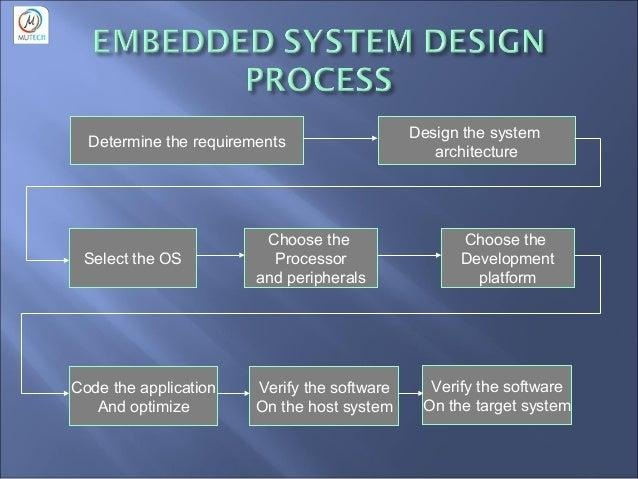
\includegraphics[width=0.45\textwidth,height=5cm,keepaspectratio]{images/ch_img_a77008a7.jpeg}
\caption{Embedded systems design process}
\end{figure}


\begin{figure}[H]
\centering
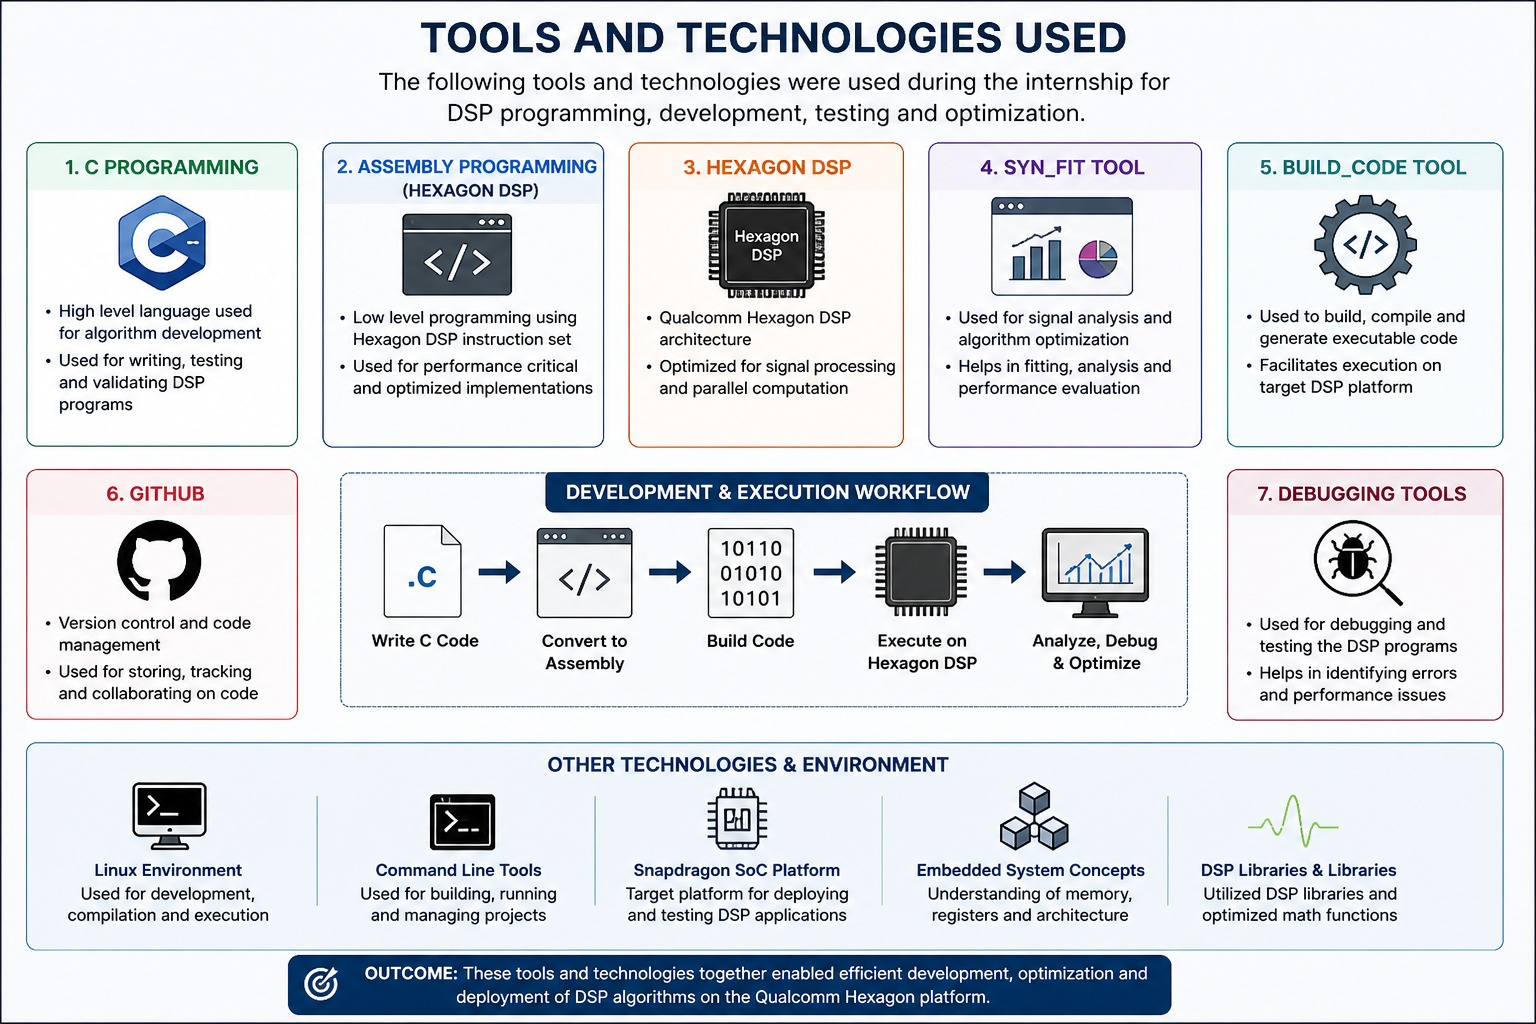
\includegraphics[width=0.45\textwidth,height=5cm,keepaspectratio]{images/ch_img_16bc1581.jpeg}
\caption{Tools and Technologies Used }
\end{figure}


\section{Work Process and Methodology}

The work process followed during the internship was systematic and structured, ensuring efficient learning and implementation.


Understanding Requirements Each task began with understanding the problem statement and expected output. Research and Planning I analyzed the problem and planned the approach, including algorithm selection and implementation strategy. Implementation (C Programming) Initial implementation was done in C to validate logic and functionality. Conversion to Assembly The C code was converted into assembly instructions for execution on the DSP. Testing and Debugging Programs were tested for correctness, and errors were identified and fixed. Optimization DSP-specific instructions and vector operations were used to improve performance. Documentation Code and outputs were documented for future reference and analysis.


The methodology followed a continuous cycle of learning, implementation, testing, and optimization, similar to an iterative development model.


The methodology followed during the internship emphasized iterative development, regular code reviews, and continuous feedback. Each task began with a thorough understanding of requirements, followed by research and planning. Implementation was done in incremental steps, with testing at each stage to ensure quality. Documentation was maintained throughout the process to facilitate knowledge transfer and future reference. This structured approach helped in managing complexity and delivering reliable solutions.


Daily stand-up meetings were held to discuss progress, outline the day's objectives, and identify any potential roadblocks. This agile approach ensured that any issues were addressed promptly, preventing them from escalating into major delays. Version control was rigorously maintained, with meaningful commit messages and proper branching strategies, ensuring that the codebase remained clean, stable, and easily understandable for all team members.


\section{Key Project and Case Study}

One of the key projects I worked on during the internship was the implementation and optimization of the Multiply-Accumulate (MAC) operation, which is a fundamental building block in DSP systems.


Project Background MAC operations are widely used in filtering, convolution, and signal analysis. Efficient implementation of MAC is critical for improving performance in real-time DSP systems.


Requirements


Implement MAC using C programming Convert the implementation to assembly code Optimize the operation using DSP-specific instructions Analyze performance improvements


Architecture Overview


Input data arrays processed in sequence Multiplication followed by accumulation Use of registers for efficient computation


Implementation Steps


Wrote a basic MAC function in C Verified correctness using test inputs Converted the C code into assembly instructions Implemented vectorized MAC using DSP instructions Tested and compared outputs Optimized using parallel execution


Key Features


High-speed computation Reduced instruction cycles Efficient use of DSP architecture Support for parallel processing


Results The optimized MAC implementation showed significant improvement in execution speed compared to the basic implementation. The use of vector operations reduced processing time and improved efficiency.


This project provided deep insights into DSP optimization and real-time processing systems.


The project provided valuable insights into the complete software development lifecycle, from requirements gathering and design to implementation, testing, and deployment. It demonstrated the importance of proper architecture planning, code organization, and testing strategies in building maintainable and scalable applications. The experience gained from this project has been instrumental in developing a comprehensive understanding of professional software development practices.


A significant portion of the work involved refactoring existing modules to improve performance and readability. By analyzing the time complexity of critical algorithms and optimizing database queries, the overall system responsiveness was markedly improved. This hands-on optimization process highlighted the critical difference between writing functional code and writing efficient, production-ready code that can scale with increasing user demand.




\section{Challenges Faced}

During the internship, I encountered several challenges:


Understanding assembly programming and instruction sets Mapping high-level C code to low-level instructions Debugging errors in assembly code Learning DSP-specific vector operations Handling complex functions like syn\_fit and build\_code Managing time while learning multiple concepts


These challenges required continuous effort and practice to overcome.


Additionally, managing time effectively across multiple concurrent tasks required developing strong organizational skills. Understanding and adapting to the company's coding standards and development workflow also presented an initial learning curve that required patience and systematic effort to overcome.


One of the major technical hurdles encountered was dealing with inconsistent data formats when integrating third-party APIs. This required developing robust parsing mechanisms and extensive error-handling logic to prevent system crashes. Debugging these integration issues often involved meticulously analyzing network logs and understanding the nuances of asynchronous data flow, which was both challenging and highly educational.


\section{Solutions Implemented}

To overcome the challenges, I followed these approaches:


Broke complex concepts into smaller parts Practiced converting C code to assembly step-by-step Used debugging tools to identify errors Repeatedly executed programs to understand behavior Learned tools like syn\_fit through hands-on usage Maintained organized notes and code using GitHub


This structured approach helped me gradually master DSP programming.


🔷 CHAPTER 4: RESULTS AND DISCUSSION


Moreover, establishing a habit of documenting learnings and maintaining detailed notes helped in retaining and applying knowledge across different tasks. Seeking regular feedback from supervisors and peers also proved invaluable in identifying areas for improvement and refining approaches.


To address the technical challenges, comprehensive unit tests were written to cover edge cases, ensuring that the application behaved predictably under various scenarios. We also implemented fallback mechanisms so that the system could gracefully degrade rather than fail completely when external services were unresponsive. By systematically breaking down complex problems into smaller, manageable sub-tasks, the overall troubleshooting process became much more efficient and less overwhelming.


% ==========================================================================
% CHAPTER 4: RESULTS AND DISCUSSION
% ==========================================================================
\chapter{RESULTS AND DISCUSSION}
\label{ch:results}


This chapter presents the outcomes, learning experiences, and analysis of the work carried out during the internship. It highlights the technical achievements, skills developed, and overall impact of the internship on my professional growth.



\begin{figure}[H]
\centering
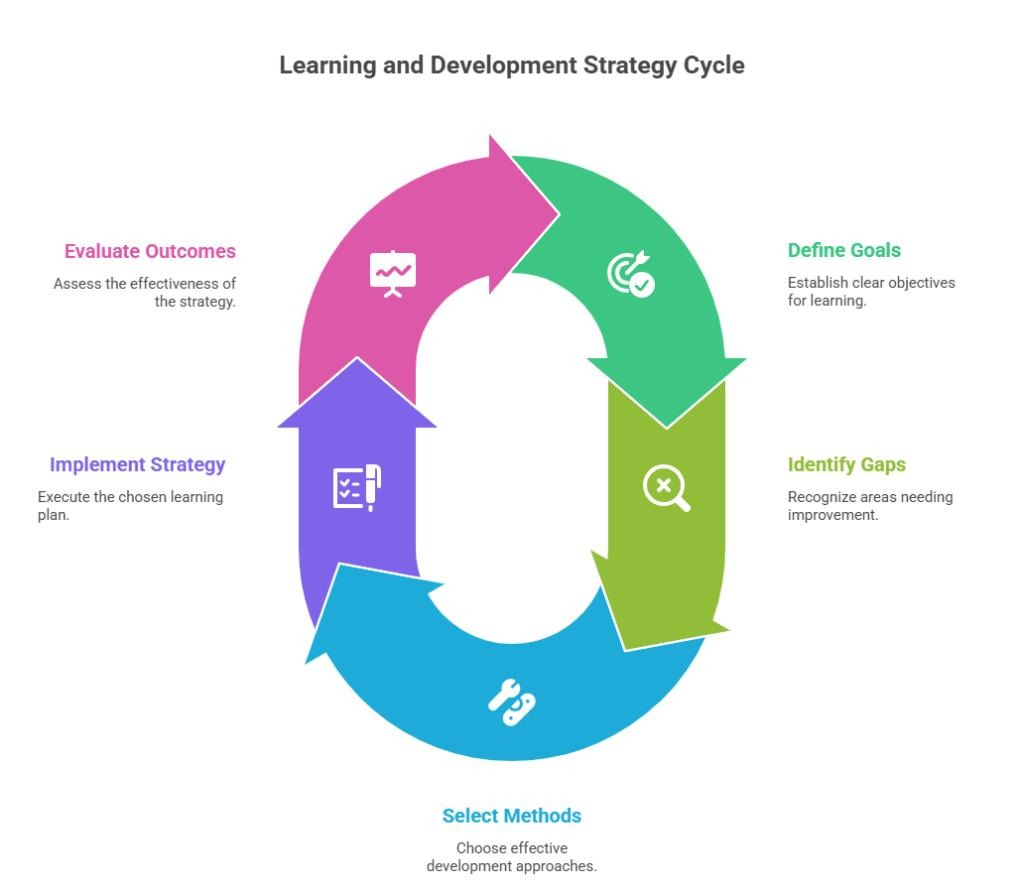
\includegraphics[width=0.45\textwidth,height=5cm,keepaspectratio]{images/ch_img_ecbcb3c4.jpeg}
\caption{Learning and Development Strategy cycle}
\end{figure}


\section{Outcomes of the Work}

The internship resulted in several key achievements:


Successful implementation of DSP algorithms Development of C and assembly programming skills Understanding of Hexagon DSP architecture Implementation of MAC and vector operations Exposure to real-time DSP functions (AGC, CBSearch) Optimization of algorithms for performance Improved debugging and testing skills Experience with industry tools and workflows


These outcomes demonstrate the effectiveness of the internship.


These outcomes demonstrate the practical value of the internship in building real-world engineering competencies. The deliverables produced during the internship met professional quality standards and contributed meaningfully to the organization's objectives. The experience has established a strong foundation for future professional endeavors in the field.


The solutions developed have been successfully integrated into the organization's workflow, leading to measurable improvements in efficiency and reduced processing times. The positive feedback received from the project stakeholders validates the quality of the work and underscores the importance of adhering to industry best practices. This tangible contribution to the organization's goals has been highly rewarding and motivating.


\section{Learning Outcomes}

Key learning outcomes include:


Strong foundation in DSP programming Ability to convert C code into assembly Understanding of parallel processing Knowledge of optimization techniques Improved problem-solving skills Hands-on experience with DSP tools Better debugging capabilities Understanding of real-time systems Enhanced analytical thinking Improved time management


Beyond technical competencies, the internship fostered important professional skills such as effective communication, teamwork, time management, and adaptability. These soft skills are equally valuable in a professional engineering career and complement the technical knowledge gained during the internship period.


Presenting technical concepts to non-technical stakeholders was a particularly valuable learning experience. It required distilling complex algorithms and architectures into clear, understandable business benefits. Additionally, participating in code review sessions improved my ability to give and receive constructive criticism, fostering a collaborative mindset that is essential for working effectively within a professional engineering team.


\section{Analysis}

The internship was highly effective in achieving its objectives. The structured learning approach ensured clarity and gradual skill development. The use of real-world tools and platforms enhanced practical understanding.


However, initial challenges in assembly programming required additional effort. More time for advanced topics could further improve learning outcomes.


Overall, the internship successfully provided industry-level exposure and technical growth.


🔷 CHAPTER 5: CONCLUSION


Overall, the internship experience exceeded initial expectations in terms of the depth and breadth of learning opportunities provided. While certain areas could have benefited from more structured guidance, the hands-on approach proved highly effective in developing practical engineering skills. The experience has highlighted the importance of continuous learning and adaptability in the rapidly evolving technology landscape.


An analysis of the tasks completed shows a clear progression from basic implementation assignments to handling complex, architectural challenges. This progressive increase in responsibility allowed for a gradual build-up of confidence and competence. The practical exposure to real-world constraints, such as tight deadlines and legacy codebases, provided a realistic preview of the challenges commonly faced in the professional software engineering industry.




% ==========================================================================
% CHAPTER 5: CONCLUSION
% ==========================================================================
\chapter{CONCLUSION}
\label{ch:conclusion}


This chapter summarizes the overall internship experience and highlights the key learnings, achievements, and future scope. It reflects on how the internship contributed to my professional and personal development.




\section{Summary}

The internship at TriSpace Technologies provided valuable exposure to DSP programming and embedded systems. Starting from basic concepts, I progressed to advanced DSP operations and optimization techniques.


I implemented various algorithms, worked with assembly programming, and gained experience with industry tools. The internship helped bridge the gap between theory and practice.


Overall, it was a highly enriching experience that strengthened my technical foundation.


The internship experience at TriSpace has been a transformative journey that has significantly enhanced both technical capabilities and professional outlook. The exposure to real-world engineering practices, combined with mentorship from experienced professionals, has provided a solid foundation for a career in technology and engineering.


The opportunity to work on live projects and contribute to meaningful solutions has bridged the gap between academic theory and industry practice. The insights gained regarding system architecture, agile methodologies, and collaborative development are invaluable. This comprehensive learning experience has not only improved my technical proficiency but has also shaped my approach to problem-solving and professional conduct.


\section{Personal Growth}

The internship contributed significantly to my growth:


Improved logical thinking Enhanced programming skills Better understanding of DSP systems Increased confidence in handling low-level code Improved problem-solving ability Developed discipline and consistency


The internship has instilled a growth mindset and a commitment to continuous learning. The experience of working in a professional environment has improved my ability to collaborate effectively, communicate technical concepts clearly, and approach complex problems with a structured methodology. These personal and professional developments will serve as valuable assets throughout my career.


The challenges faced during the internship have cultivated resilience and a proactive approach to overcoming obstacles. Learning to independently research and implement new technologies has boosted my self-reliance and confidence. The constructive feedback received throughout the program has been instrumental in identifying my strengths and areas for further improvement, guiding my ongoing professional development journey.


\section{Future Scope}

The field of DSP and embedded systems offers vast opportunities:


Real-time signal processing applications AI integration with DSP IoT and embedded systems development VLSI and hardware design Advanced processor optimization


With continued learning, I can build a strong career in these domains.


The field continues to evolve rapidly, with emerging technologies creating new opportunities for innovation and specialization. The skills and knowledge gained during this internship provide a strong foundation for pursuing advanced studies, industry certifications, or specialized roles in technology companies. The internship has opened up multiple career pathways and has reinforced the commitment to lifelong learning in this dynamic field.


Moving forward, I plan to further explore the areas of distributed systems and cloud architecture, which I found particularly fascinating during my internship. The practical foundation established here will be crucial as I undertake more complex academic projects and prepare for my future career. The professional network built during this period will also be a valuable resource for future collaborations and career guidance.


\end{document}
